\providecommand{\main}{../../../..}
\documentclass[\main/dresen_thesis.tex]{subfiles}
\begin{document}
  \label{sec:doubleLayers:vsm}

  \begin{figure}[tb]
    \centering
    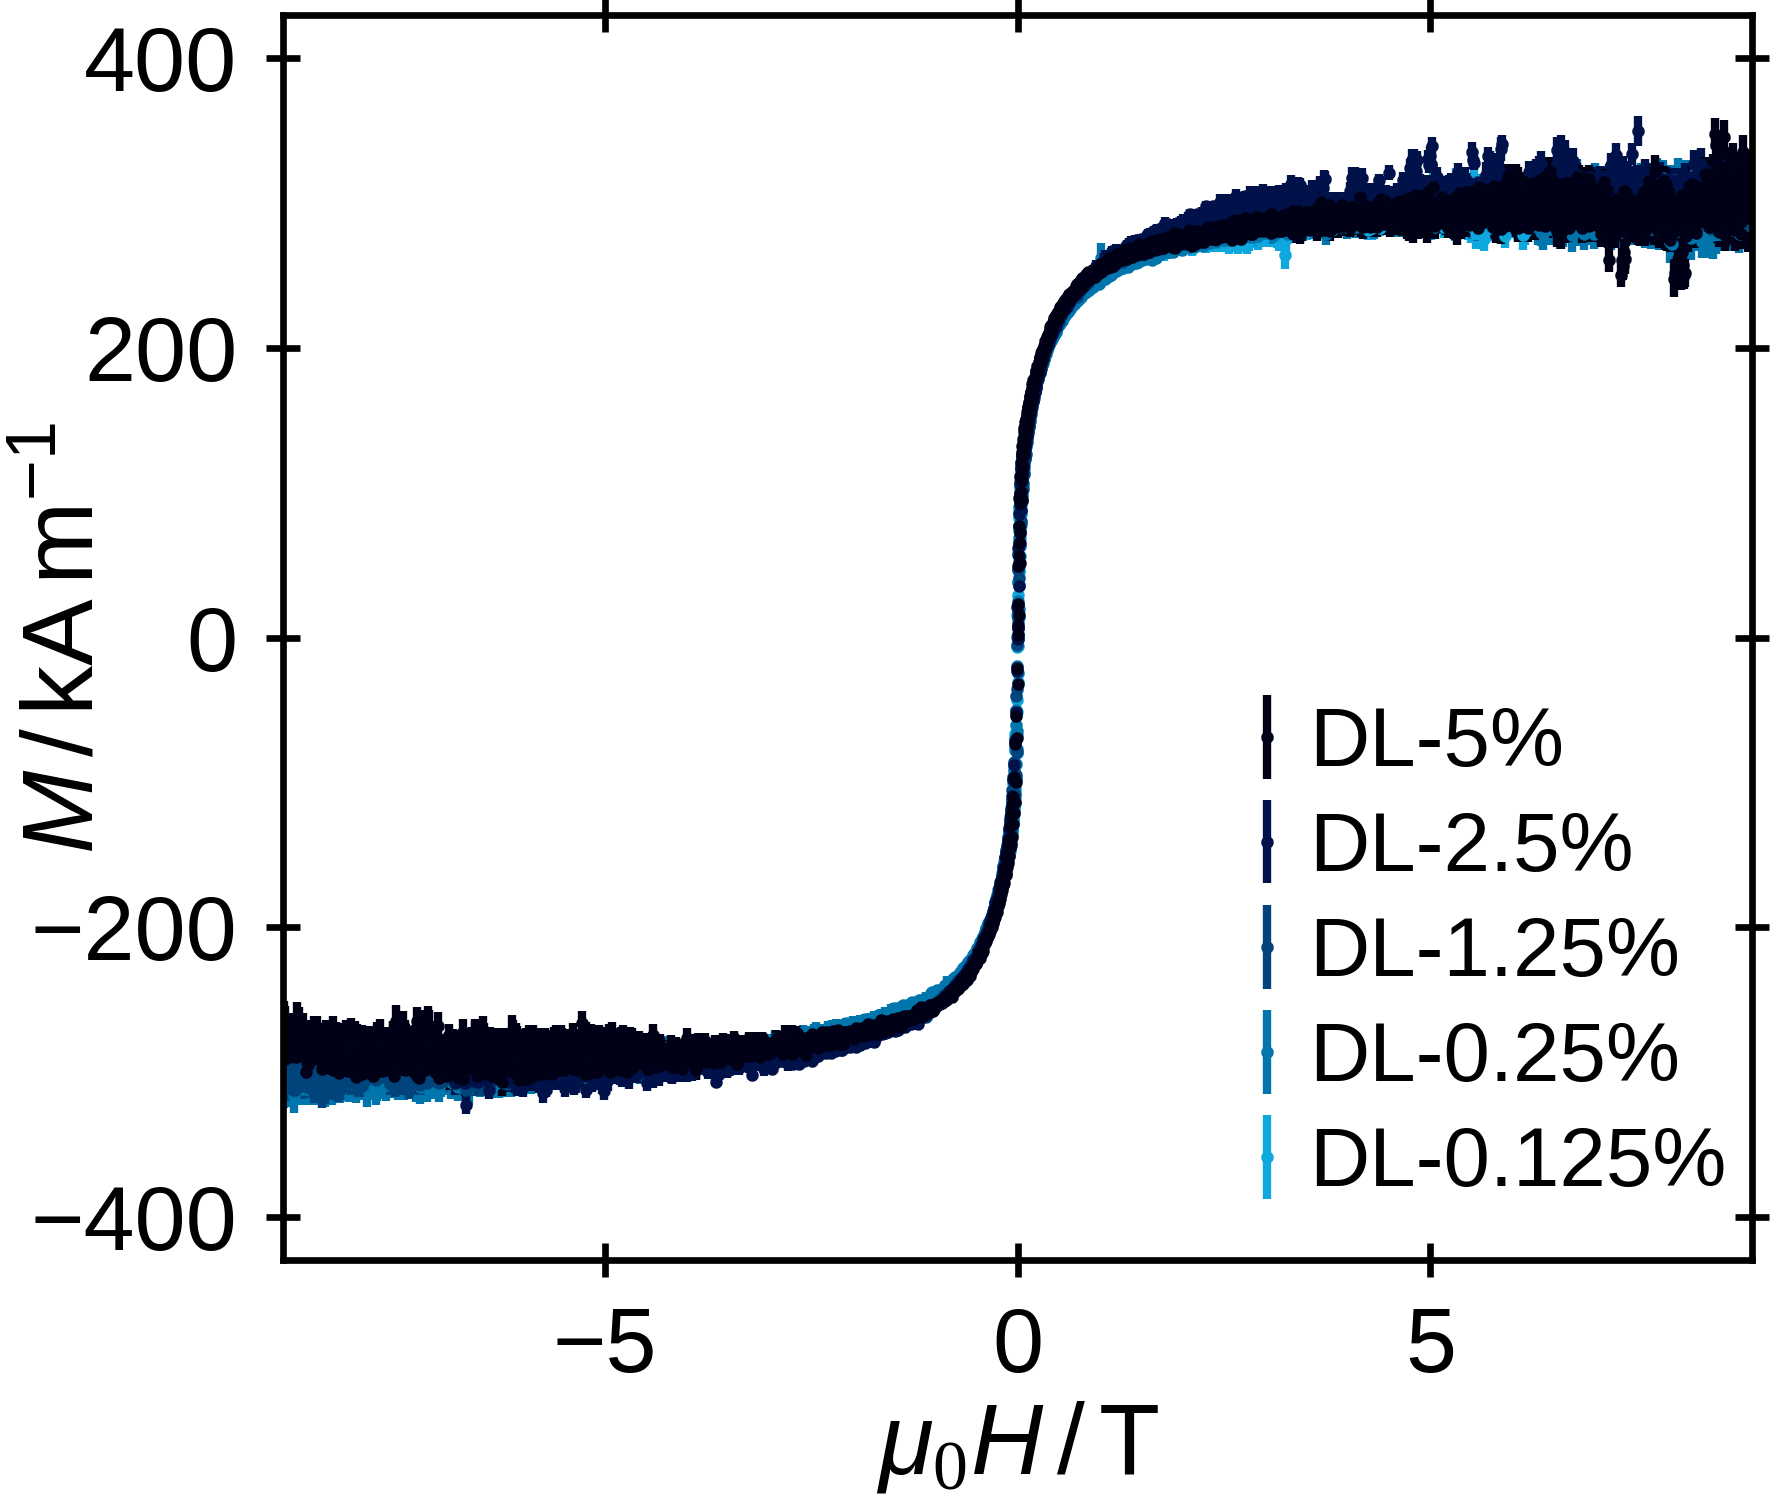
\includegraphics{doublelayers_PPMS_300K_allSamples}
    \caption{\label{fig:doubleLayers:RTVSM}Room temperature field-dependent magnetization of the double layer samples. The magnetizations are shifted with respect to each other for direct comparison. The data is corrected for the susceptibility and scaled to the observed spontaneous magnetization given in \reftab{tab:doubleLayers:RTVSM:parameters}.}
  \end{figure}

  \paragraphNewLine{Scaling of the Data and Silicon Background}
    Each double layer has been measured field- and temperature-dependent with the same procedure and conditions for direct comparison of the magnetic properties.
    As each double layer sample is prepared from the same dispersion and with a similar procedure, differences in the magnetic properties should be attributable to dipolar interlayer coupling as the PMMA thickness is the only varied parameter.
    Slight deviations are given in the sample size that is measured in the VSM due to the finite precision in breaking of the sample.
    In \reftab{tab:doubleLayers:RTVSM:parameters}, the determined susceptibility $\tilde{\chi}$ and spontaneous magnetization $\tilde{M}_s$ obtained from the room temperature measurements by a linear fit in the range of $5 - 9 \unit{T}$ is tabulated.
    As the magnetic samples are assumed to be all two layers of nanocubes and the susceptibility should be given by the size of the silicon substrate, the variation in the spontaneous magnetization and susceptibility should only be given by the variation of the sample size.
    Therefore, the values are also shown as scaled to the varied sample mass, which accounts for the different cut sizes.

    \begin{table}[!htbp]
      \centering
      \caption{\label{tab:doubleLayers:RTVSM:parameters} Spontaneous magnetization and susceptibility of the raw double layer magnetization determined by fitting the slope of the data in the range of $5 - 9 \unit{T}$.}
      \begin{tabular}{ l | l | l | l | l}
        \rule{0pt}{2ex} \textbf{VSM @ 300 K}  & $\tilde{M}_s \, / \unit{\musf emu}$ & $\bar{M}_s \, / \unit{\musf emu / mg}$ & $\tilde{\chi} \, / \unit{\musf emu \, T ^{-1}}$ & $\bar{\chi} \, / \unit{\musf emu \, T ^{-1} mg^{-1}}$ \\
        \hline
        \rule{0pt}{2ex} DL-0.125\%   & $87.2(2)$   & $2.95(1)$   & $-36.96(3)$ & $-1.251(1)$\\
        \rule{0pt}{2ex} DL-0.25\%    & $83.6(3)$   & $3.05(1)$   & $-35.58(4)$ & $-1.297(1)$\\
        \rule{0pt}{2ex} DL-1.25\%    & $87.4(2)$   & $3.27(1)$   & $-33.78(3)$ & $-1.264(1)$\\
        \rule{0pt}{2ex} DL-2.5\%     & $86.5(5)$   & $2.93(2)$   & $-36.02(7)$ & $-1.221(2)$\\
        \rule{0pt}{2ex} DL-5\%       & $90.2(5)$   & $2.98(2)$   & $-39.78(8)$ & $-1.314(3)$\\
        \hline
      \end{tabular}
    \end{table}

    For the rescaled values, the mean susceptibility is $-1.269\, / \unit{\musf emu \, T ^{-1} mg^{-1}}$ with a relative standard deviation of $3.7 \%$  and the mean spontaneous magnetization is $3.036 \, / \unit{\musf emu / mg}$ with a relative standard deviation of $4.5 \%$.
    The susceptibility can be compared to the theoretical value of pure silicon, which is $-1.11\, / \unit{\musf emu \, T ^{-1} mg^{-1}}$ \cite{Lide_2004_Handb}.
    The higher value and fluctuations of the susceptibility after scaling to the silicon mass accounts for the varnish used to fix the sample, which is of varying amount.
    For the spontaneous magnetization the fluctuations after scaling to the silicon mass tells that slight variations are given in the nanocube content in each double layer.
    This is connected to the finite precision of the pipettes that are used to transfer the nanocubes from dispersion to the substrate during drop casting.

    As no strong interaction effects are expected at room temperature, the samples are scaled using the measured spontaneous magnetization, such that relative changes after cooling to low temperatures can become more visible.
    The diamagnetic contributions are also subtracted from the data, as they are arguably a pure signal from the silicon substrate.
    The resulting room temperature magnetizations that closely resemble each other after correction are shown in \reffig{fig:doubleLayers:RTVSM}.
    The determined scaling factors by the spontaneous magnetization and the same diamagnetic correction are applied to the low temperature field-dependent and temperature-dependent measurements without further modification.

  \begin{figure}[tb]
    \centering
    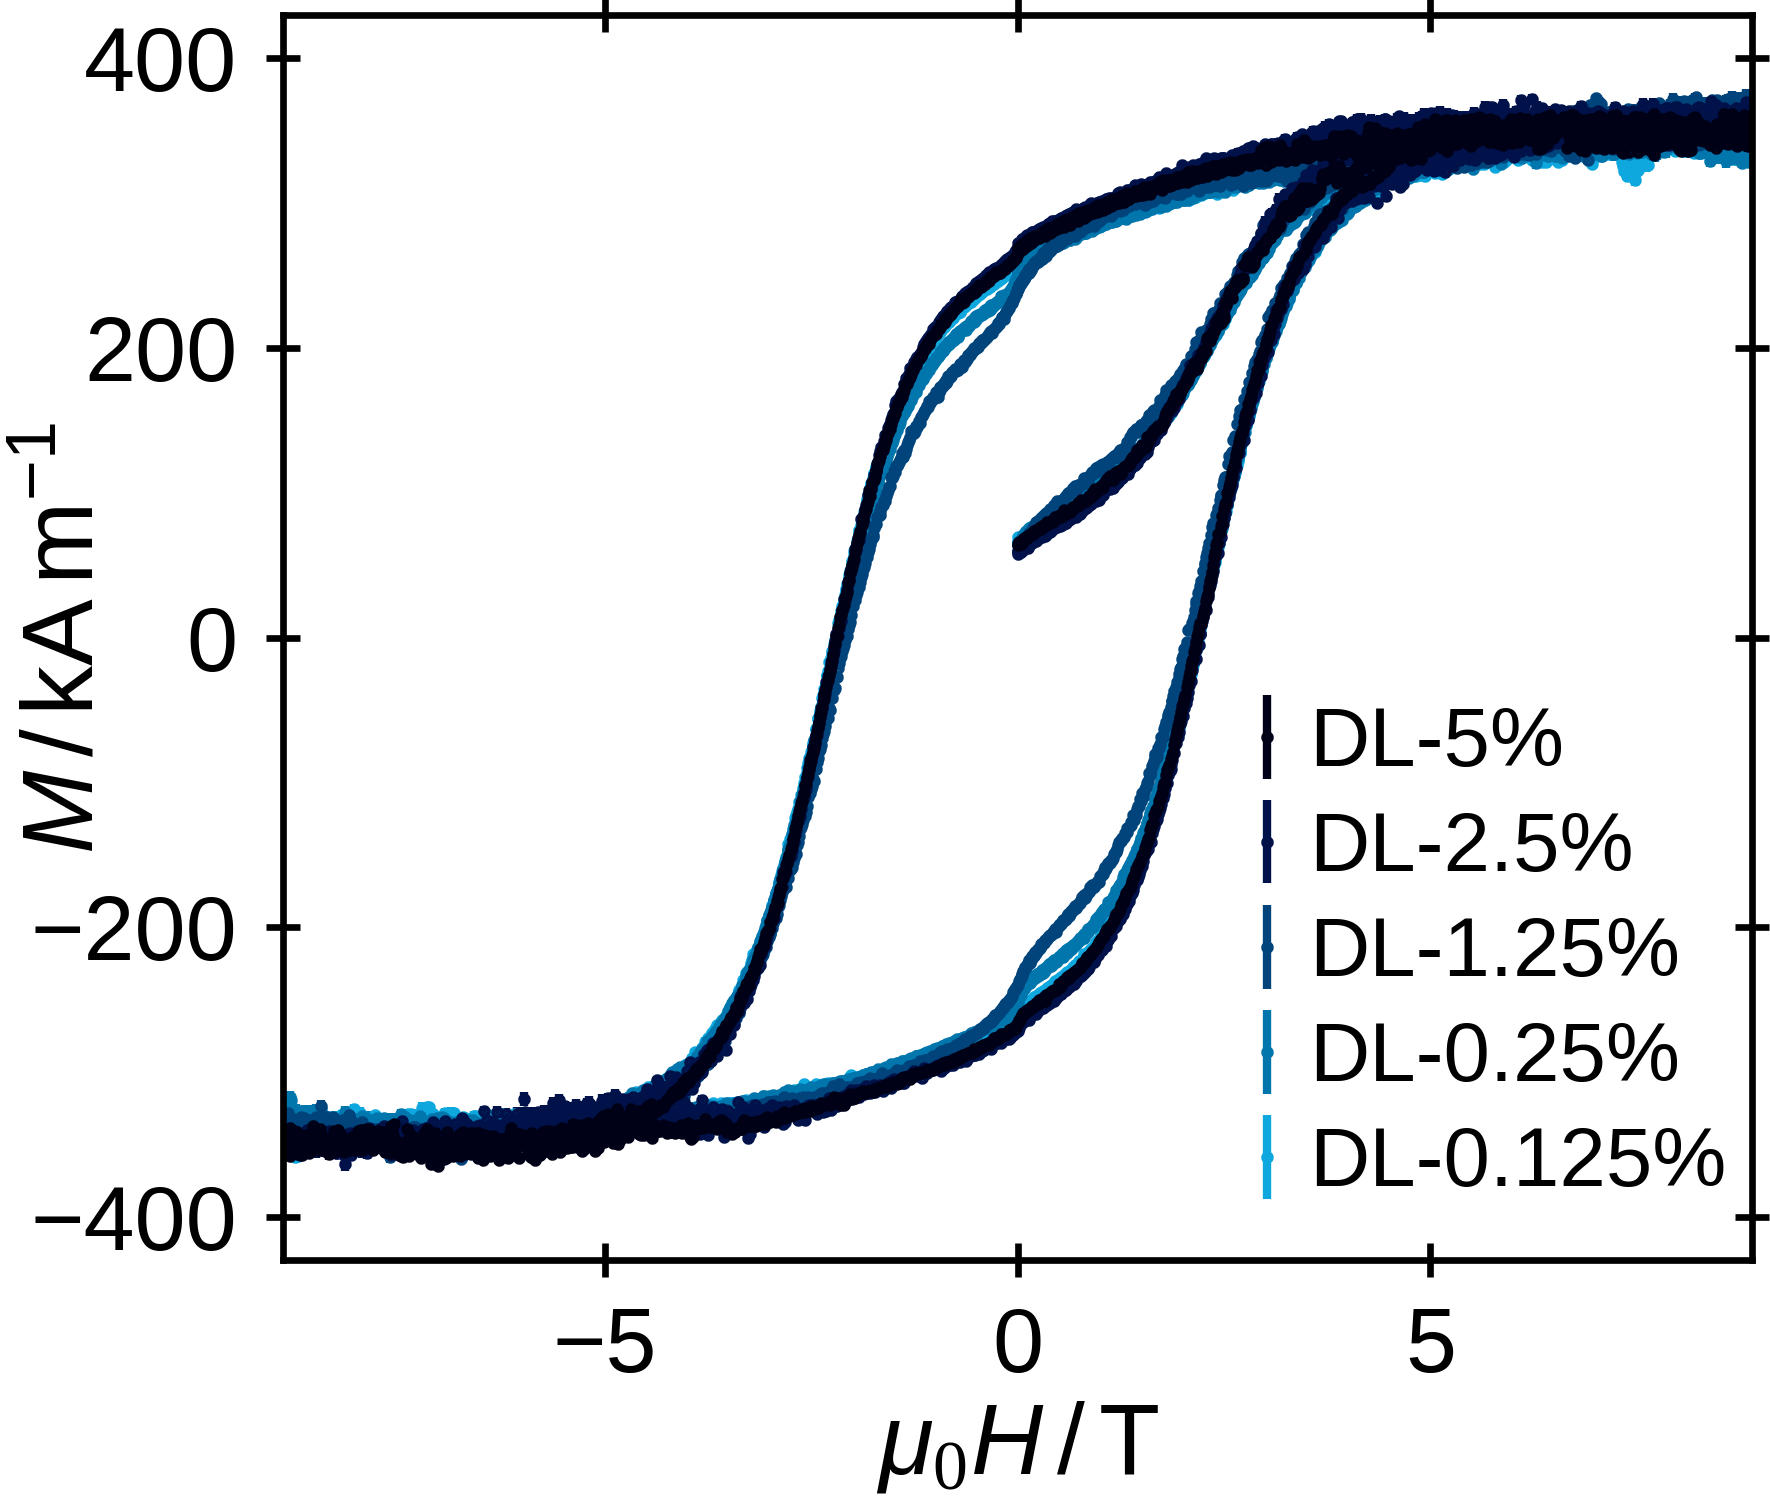
\includegraphics{doublelayers_PPMS_10K_allSamples}
    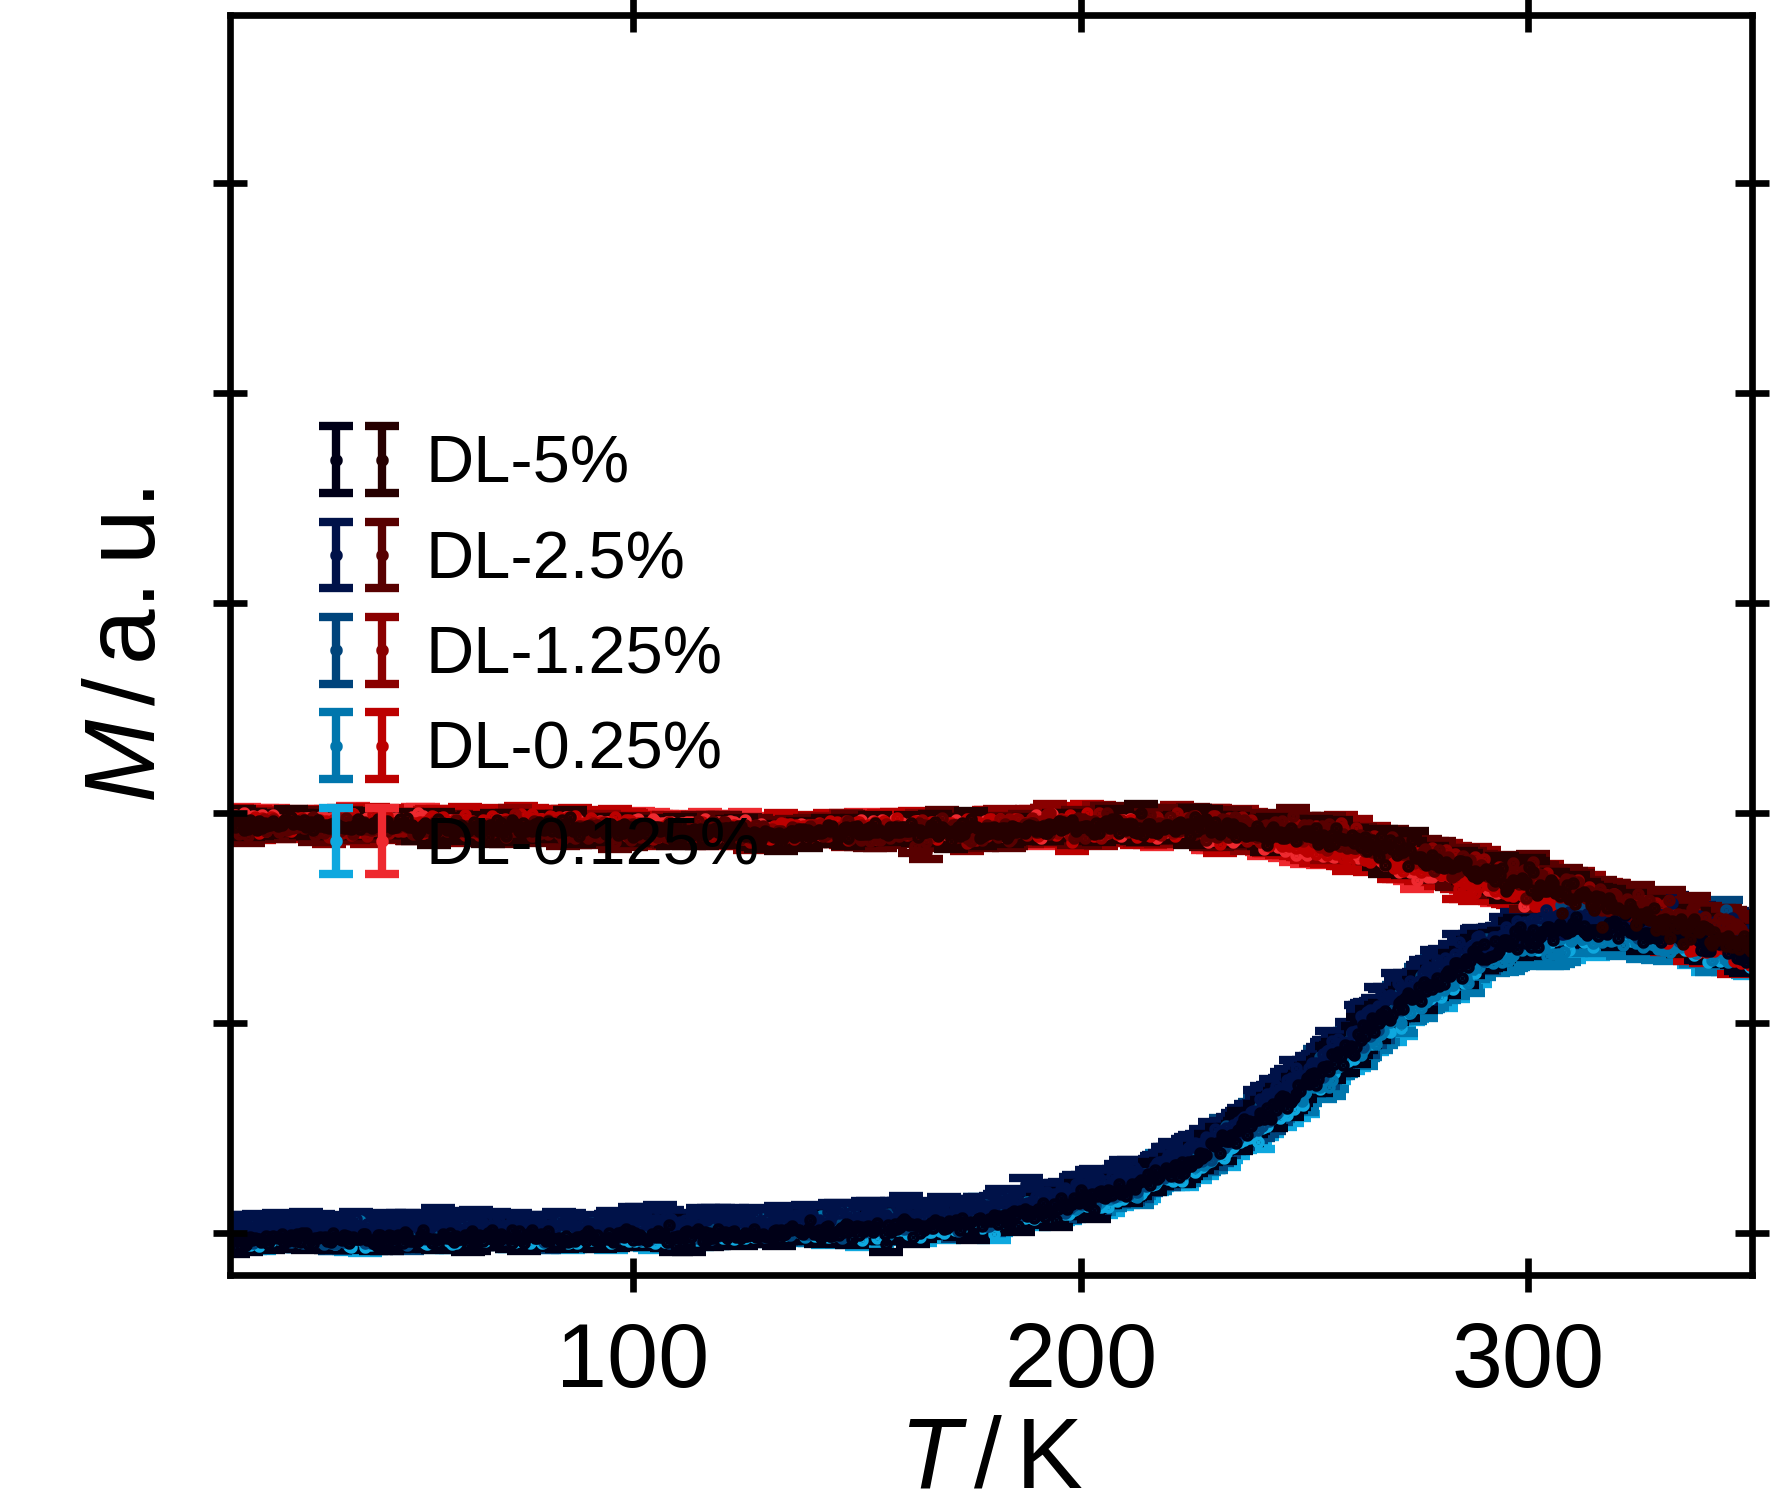
\includegraphics{doublelayers_PPMS_ZFC_FC_allSamples}
    \caption{\label{fig:doubleLayers:zfcFCData}Field- (left) and temperature-dependent (right) magnetization of the double layers. The hysteresis are each measured at a temperature of $10 \unit{K}$ after cooling in zero field, and the temperature-dependent ZFC/FC magnetizations are taken with a field of $10 \unit{mT}$ while warming the sample.  To discuss the qualitative differences, the zero-field cooled and field cooled data, as well as the respective data of the samples with varied spacer thicknesses are shifted by a constant factor.}
  \end{figure}

  \paragraphNewLine{Temperature-dependent magnetization}
    In \reffig{fig:doubleLayers:zfcFCData} the temperature-dependent magnetization is shown for the double layer samples, sorted with respect to the varied PMMA thickness.
    A close inspection of temperature dependent magnetization shows that they all closely resemble each other and no significant difference can be observed across the samples.
    Similar to the monolayer sample in \refsec{sec:monolayers:magneticStructure:vsm}, a blocking temperature around $315 \unit{K}$ is observed as peak temperature in the zero-field cooled magnetization.
    No major shift in that peak position can be observed within the resolution of the measurement, which could otherwise have been a sign for interlayer interaction.

  \paragraphNewLine{Field-dependent low temperature magnetization}
    Subtle differences can however be seen in the hysteresis at $10 \unit{K}$.
    Similar to the monolayer sample, a small jump in the magnetization is visible around $\pm 100 \unit{mT}$.
    The strength is visibly changing from sample to sample, without showing a systematic with respect to the PMMA layer thickness.
    Whereas it appear to be nearly invisible for the lowest PMMA concentration sample DL-0.125\%, it appears clearly visible for DL-0.25\%, reduces in size for DL-1.25\% and becomes stronger again for DL-2.5\%.
    As one would expect from dipolar coupling a reduction of interaction effects with increasing layer thickness and as the jump also appears in monolayer samples, it is probable that this effect is not directly correlated to dipolar interlayer interaction but an uncontrolled property of the nanocube arrays themselves.
    Otherwise the hysteresis resemble each other closely, where each has a coercive field in the magnitude of $2.16(3) \unit{T}$, in agreement with the monolayer sample.
  % In literature, the jump can be found in multiple works discussing cobalt ferrite nanoparticles \cite{Xu_2015_Simul, Fu_2012_Uniqu, Lima_2017_Waspw}.
  % The authors give multiple explainations ranging from dipolar interaction between the particles, to surface spin reorientation, o
  % At the state of this thesis it is yet unclear what the true nature of the jump at low fields is.

  

  % \begin{table}[!htbp]
  %   \centering
  %   \caption{\label{tab:looselyPackedNP:nanoparticle:gisaxs}Parameters for the hard-sphere structure factor in Percus-Yervick approximation shown in for both SC-IOS-11 and SC-IOS-7. $R_\mathrm{HS}$ is the hard-sphere radius and $\eta$ the packing fraction of the structure factor.}
  %   \begin{tabular}{ c | l | l }
  %     \rule{0pt}{2ex} \textbf{GISAXS}  & \textbf{SC-IOS-11} & \textbf{SC-IOS-7} \\
  %     \hline
  %     \rule{0pt}{2ex} $R_\mathrm{HS} \, / \unit{nm}$          & $5.655(2)$           & $3.872(4)$\\
  %     \rule{0pt}{2ex} $\eta          \, / \unit{\%}$          & $43.88(3)$           & $34.20(9)$\\
  %     \hline
  %   \end{tabular}
  % \end{table}
\end{document}